% Chapter Template

\chapter{Reti Neurali Convoluzionali} % Main chapter title
\label{Capitolo3}
\def \teoria {Figures/teoria}
\def \path	 {Figures/C3}
%--------------------------------------------------------------------%	SECTION 1
%--------------------------------------------------------------------
%% da completare
In questo capitolo si introduce una panoramica generale sulle reti neurali convoluzionali. Essendo un argomento vasto, una trattazione teorica approfondita sarebbe materia di una tesi di laurea, ragion per cui gli argomenti sono introdotti con lo scopo di avere un'infarinatura per comprendere le applicazioni sviluppate nei capitoli successivi. 
\section{Breve introduzione}
La reti neurali convoluzionali, alle quali ci riferiremo con l'abbrevazione \emph{CNN} - dall'inglese \emph{Convolutional Neural Network}, sono un'evoluzione delle normali reti artificiali profonde caratterizzate da una particolare architettura estremamente vantaggiosa per compiti visivi e non, che le ha rese negli anni molto efficaci e popolari. Ispirate 

%%% ricollocare la figura %%% 
\begin{figure}[h!]
 \centering
 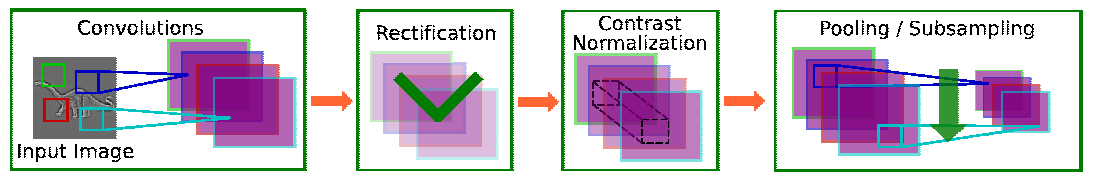
\includegraphics[width=1.0\textwidth]{\path/CNN-features.png} 
 \caption{I diversi strati tipici di una CNN}
 \label{fig:conv1}
\end{figure}

%--------------------------------------------------------------------
%	SECTION 2
%--------------------------------------------------------------------

\section{Architettura}
\subsection{Strato di Convoluzione}

\subsection{Strato di Pooling}

\subsection{Strato completamente connesso (FC)}


%--------------------------------------------------------------------
%	SECTION 3
%--------------------------------------------------------------------

\section{Applicazioni e risultati}


